
\section{Expérimentations}

Dans cette section, nous évaluons l'impact de l'adaptabilité de \SPRAY sur les
métriques communément employées dans l'étude des performances de protocoles
d'échantillonnage de pairs. Ceux-ci incluent le coefficient de clustering, la
taille moyenne du plus petit chemin, la distribution du nombre de connexions
entrantes, le nombre d'arcs, et les composantes connexes. \CYCLON constitue
l'approche à taille fixe avec laquelle nous comparerons les résultats en lien
avec l'adaptabilité. Les résultats attendus sont :
\begin{inparaenum}
\item des propriétés identiques pour les deux approches lorsque \CYCLON est
  configuré de manière optimale,
\item une meilleure efficacité de \SPRAY lorsque les vues partielles de \CYCLON
  sont trop grande par rapport à la taille du réseau,
\item une plus grande robustesse lorsque les vues partielles de \CYCLON sont
  trop petites par rapport à la taille du réseau.
\item Enfin, contrairement à \CYCLON, \SPRAY possède des doublons dans ses vues
  partielles. Toutefois, ce nombre de doublons est supposé négligeable.
\end{inparaenum}
\SCAMP constitue l'approche avec laquelle nous comparerons \SPRAY lorsque nous
examinerons les échecs dans l'établissement des connexions. Nous nous attendons
à ce que \SCAMP échoue à maintenir un réseau connecté, contrairement à \SPRAY.

Les expérimentations ont été exécuté sur le simulateur
\PEERSIM~\cite{montresor2009peersim}. Le code relatif aux protocoles
d'échantillonnages \CYCLON, \SCAMP, et \SPRAY sont disponibles sur la
plate-forme Github\footnote{\url{http://github.com/justayak/peersim-spray}}.

\begin{figure*}
  \centering
  \subfloat[Figure A][Clustering coefficient of \CYCLON.]{
    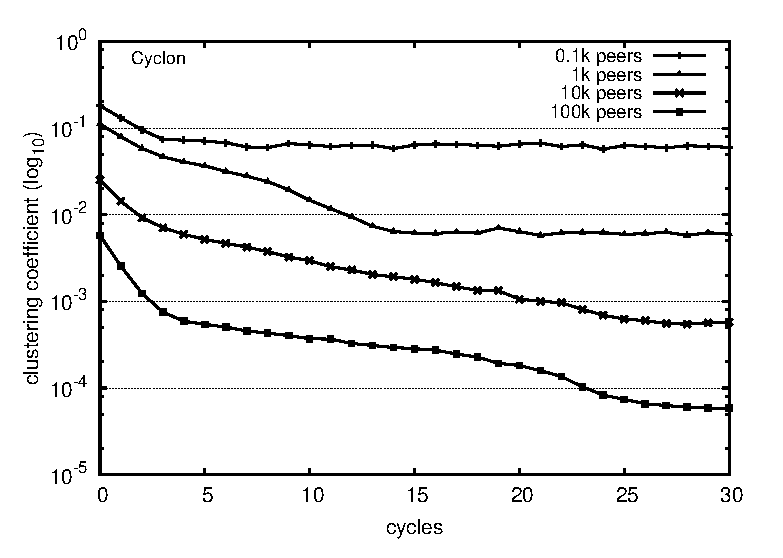
\includegraphics[width=0.47\textwidth]{img/spray/cycloncluster.eps}}
  \hspace{10pt}
  \subfloat[Figure B][Clustering coefficient of \SPRAY.]{
    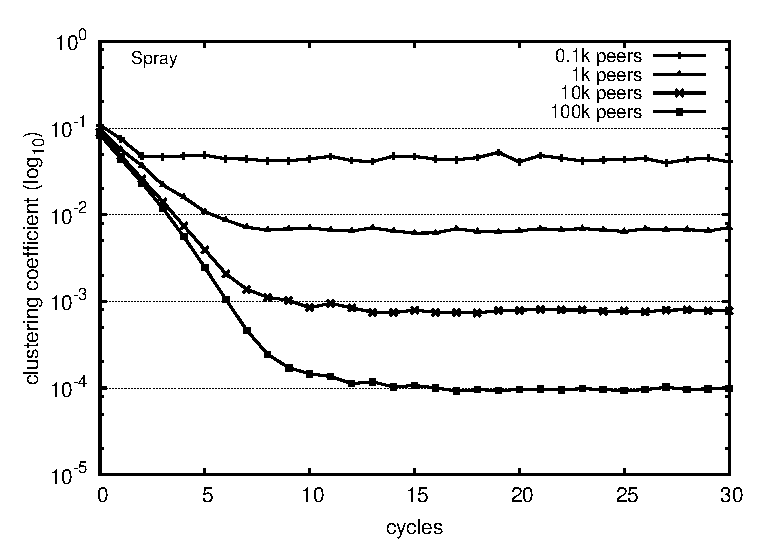
\includegraphics[width=0.47\textwidth]{img/spray/spraycluster.eps}}
  \caption{\label{fig:spray:clustering}The x-axis denotes the elapsed time in
    cycles while the y-axis denotes the $\log_{10}$-scaled clustering
    coefficient.}
\end{figure*}

\begin{asparadesc}
\item [Objectif:] Montrer comment l'adaptabilité influence le clustering et le
  temps de convergence.
\item [Description:] Le coefficient de clustering moyen $\overline{C}$ mesure la
  connexité du voisinage de chaque pair dans le réseau :
  \begin{equation}
    \overline{C} = {1\over |\mathcal{N}|}\sum\limits_{x\in\mathcal{N}}C_x
  \end{equation}
  où $C_x$ est le coefficient de clustering local du pair $p_x$. L'expérience
  implique 0.1k, 1k, 10k, et 100k pairs. Le représentant des approches à taille
  fixe est \CYCLON. Ce dernier est configuré de manière optimale pour 1k pairs
  ($\ln(1000)\approx 7$ voisins). Durant les échanges, les pairs utilisant
  \CYCLON mélangent 3 de leurs 7 voisins. Ainsi, les vues partielles de \CYCLON
  sont trop grandes pour 0.1k pairs, et trop petites pour 10k et 100k pairs.
\item [Résultat:] La figure~\ref{fig:spray:clustering} montre que \CYCLON
  démarre avec un coefficient de clustering plus bas que \SPRAY. Malgré cela,
  \SPRAY parvient à converger plus rapidement que \CYCLON. De plus, quand le
  nombre de pairs augmente dans le réseau, le temps de convergence de \CYCLON en
  souffre fortement. À l'opposé, \SPRAY converge très rapidement quel que soit
  la taille du réseau. La figure~\ref{fig:spray:clustering} montre aussi que les
  deux approches convergent vers un coefficient de clustering bas
  caractéristique des graphes aléatoires. Néanmoins, \CYCLON et \SPRAY
  n'atteignent pas les mêmes valeurs après convergence. À l'exception du cas où
  \CYCLON est configuré de manière optimale, les valeurs obtenus par \SPRAY sont
  soit au dessous (lorsque les vues de \CYCLON sont trop grandes) ou au dessus
  (lorsque les vues de \CYCLON sont trop petites). Globalement, cela montre que
  \SPRAY
  \begin{inparaenum}[(i)]
  \item converge vers un coefficient de clustering stable,
  \item qui reflète les besoins dû à la taille du réseau.
  \end{inparaenum}
  Cela a une influence sur l'équilibrage des charges et la robustesse par
  rapport aux allées et venues de pairs.    
\item [Explications:] \CYCLON commence avec un coefficient de clustering plus
  petit car lorsqu'un pair rejoint le réseau, un cheminement aléatoire est
  effectué afin d'en faire l'annonce. Ainsi, le réseau de départ est déjà
  légèrement équilibré au moment où la simulation commence les échanges de vue
  partielle. À l'opposé, un nouvel arrivant avec \SPRAY n'annonce son entrée
  qu'au voisinage de son contact. De ce fait, le réseau est fortement
  déséquilibré au départ de l'expérience, quelle que soit taille du
  réseau. Malgré cela, \CYCLON ne converge pas aussi vite que \SPRAY vers un
  coefficient stable. Cela est due à la taille fixe de sa vue partielle qui
  contraint la qualité des échanges. Le coefficient de clustering mesure la
  connexité du voisinage de chaque pair dans le réseau. Cela dépend donc de la
  taille de vue partielle qui, pour \CYCLON, est fixé lors de la configuration.
  Ainsi lorsque le nombre de pairs est multiplié par 10, le coefficient de
  clustering est divisé par 10. En revanche, les pairs utilisant \SPRAY ont une
  taille de vue partielle pouvant varier afin de refléter la taille du réseau.
  Ainsi, quand le réseau contient 1k pairs, les vues partielles s'adaptent à
  cette taille. Par conséquent, \SPRAY est très légèrement en dessous de \CYCLON
  dans ce scénario car la taille moyenne de vue partielle est de 7.4 pour ce
  premier contre 7 pour ce second. En étendant ce raisonnement aux autres
  tailles de réseau, cela explique pourquoi \SPRAY converge vers une valeur plus
  basse lorsque les vues partielles de \CYCLON sont trop grandes, et vers une
  valeur plus haute lorsque les vues partielles de \CYCLON sont trop petites.
\end{asparadesc}

\begin{figure}
  \centering
  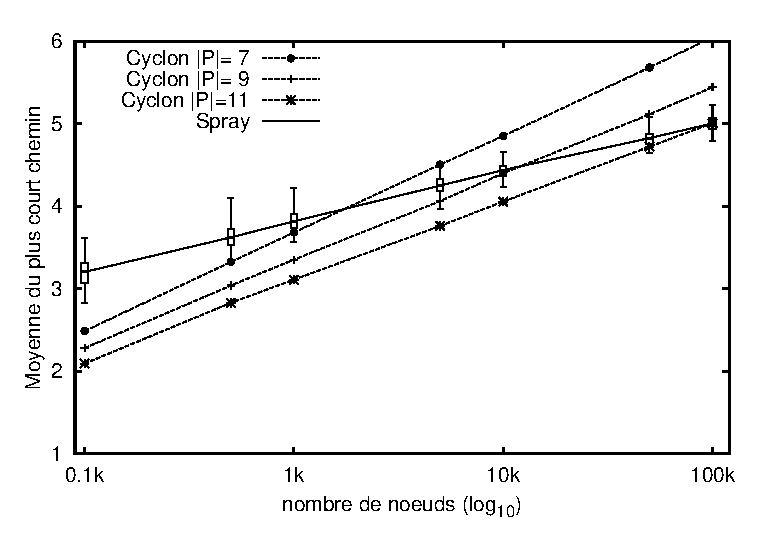
\includegraphics[width=.8\textwidth]{img/spray/avgpath.eps}
  \caption{\label{fig:spray:avgpath}The average shortest path length of \SPRAY
    and \CYCLON. The x-axis denotes the number of peers in the network on a
    $\log_{10}$ scale (from 100 to 100k peers) while the y-axis denotes the
    average shortest path length of the network.}
\end{figure}

\ \\

\begin{asparadesc}
\item [Objectif:] Observer comment l'adaptabilité influence la taille du plus
  court chemin moyen, i.e., l'efficacité de la dissémination d'informations.
\item [Description:] La taille du plus petit chemin moyen est calculée en
  comptant le nombre de sauts (de voisin en voisin) d'un pair pour parvenir à
  tous les autres pairs. En d'autres termes, cette métrique indique le temps
  qu'une information, sous la forme d'un message, peut voyager et atteindre tous
  les pairs au moins une fois. Afin d'effectuer la moyenne, nous choisissons
  aléatoirement un sous-ensemble de pairs appartenant au réseau. Ce procédé est
  répété sur 100 exécutions afin d'éviter tous les effets de bord dus à
  l'indéterminisme des protocoles d'échantillonnages. Les expérimentations
  concernent \CYCLON configurés de façon optimale pour différentes tailles de
  réseau. Le \CYCLON avec une taille de vue partielle de 7 cible environ 1.1k
  pairs. Le \CYCLON avec une taille de vue partielle de 9 cible environ 8.1k
  pairs. Le \CYCLON avec une taille de vue partielle de 11 cible environ 60k
  pairs. Lors de toutes ces simulations, les mesures sont effectuées après
  convergence. Celles-ci sont faites lorsque la taille du réseau atteint 0.1k,
  0.5k, 1k, 5k, 10k, 50k, et 100k pairs. 
\item [Résultats:] La figure~\ref{fig:spray:avgpath} montre que \CYCLON et
  \SPRAY ont tous deux un chemin moyen relativement petit. Ainsi, les
  informations peuvent être disséminées à tous les membres du réseau très
  rapidement. La figure~\ref{fig:spray:avgpath} montre aussi que chaque
  exécution de \CYCLON prise séparément peut être divisée en trois phases.  Tout
  d'abord, la phase où les vues partielles de \CYCLON sont trop grandes
  dissémine l'information plus rapidement que \SPRAY. Lors les vues partielles
  sont optimales, \CYCLON et \SPRAY montrent des résultats similaires. Enfin,
  \SPRAY montre une meilleure efficacité lorsque les vues partielles de \CYCLON
  sont trop petites. Malgré tout, \SPRAY s'adapte mieux que \CYCLON à la taille
  du réseau car l'inclinaison de cette première est inférieure à n'importe
  quelle configuration de cette dernière.
\item [Explication:] Les mesures sont toutes effectuées après convergence,
  lorsque le réseau possède une topologie qui est proche d'un graphe aléatoire.
  Dans de tel graphe, le diamètre et la taille du plus court chemin moyen
  restent petits. La seconde observation concerne chacune des configurations de
  \CYCLON comparée à \SPRAY. Une taille de vue partielle surestimée pour \CYCLON
  est meilleure en terme de connexité entre pairs et résulte dans de plus courts
  chemins en moyenne. En revanche, dès que cette taille devient insuffisante
  pour le réseau, \SPRAY devient plus efficace car il possède de plus grandes
  vues partielles. Puisque \SPRAY suit toujours la taille optimale de vue
  partielle, il passe mieux à l'échelle en terme de taille réseau.
\end{asparadesc}

\begin{figure}
  \centering
  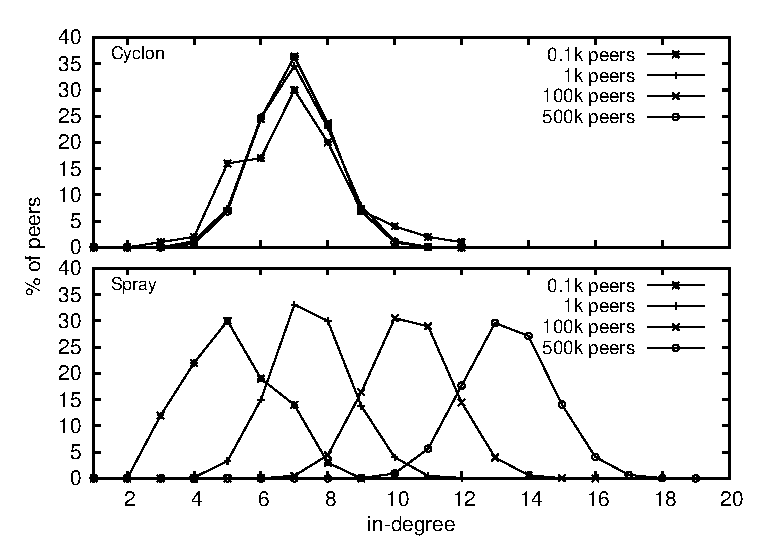
\includegraphics[width=.8\textwidth]{img/spray/histo.eps}
  \caption{\label{fig:spray:histo}The in-degree distribution of \CYCLON and
    \SPRAY. The x-axis denotes the in-degree in number of nodes while the
    y-axis indicates the percentage of peers with such in-degree. The top
    figure is dedicated to the runs concerning \CYCLON while the bottom figure
    concerns \SPRAY.}
\end{figure}

\ \\

\begin{asparadesc}
\item [Objectif:] Montrer comment l'adaptabilité influence la distribution des
  connexions entrantes, i.e., la charge parmi les pairs.
\item [Description:] Les connexions entrantes d'un pair montre à quel point ce
  pair est représenté dans les vues partielles des autres pairs. La distribution
  des connexions entrantes permet de mettre en lumière l'existence de pairs avec
  une faible connexité, et les groupes fortement liés. Cela influence
  directement la robustesse du réseau. Dans cette expérimentation, \CYCLON est
  configuré avec une vue partielle contenant 7 voisins (optimal pour 1.1k
  pairs). Les mesures sont faites après convergence avec les tailles de réseau
  suivantes: 0.1k, 1k, 100k, 500k pairs.
\item [Résultat:] Le haut et le bas de la figure~\ref{fig:spray:histo} montrent
  la distribution des connexions entrantes pour \CYCLON et \SPRAY,
  respectivement. Nous observons que \CYCLON possède une distribution identique,
  quelle que soit la taille du réseau. Ainsi, la distribution d'un réseau de
  0.1k pairs est identique à celle de 500k pairs, avec une moyenne aux environs
  de 7 et un fort pic à cette valeur. À l'opposé, la distribution des connexions
  entrantes de \SPRAY suit la taille du réseau. La figure~\ref{fig:spray:histo}
  montre aussi que les pairs sont très concentrés autour des valeurs
  moyennes. Par exemple, lors de l'exécution du protocole \SPRAY avec 500k
  pairs, la moyenne est de 13.37 avec 88\% des pairs compris entre 12 et 14
  inclus. Cela signifie que la charge est très équilibrée parmi les
  pairs. Puisque chaque pair est aussi important que son voisin en terme de
  connectivité,le réseau est résistant aux défaillances.
\item [Explication:] Une fois configuré, \CYCLON doit gérer tous les réseaux,
  quelle que soit leur taille, avec une vue partielle dont la taille est
  constante. Proportionnelement, le nombre de fois qu'un pair est référencé dans
  les vues partielles ne change pas comparé à la taille réseau. En effet, le
  nombre d'arcs qu'un pair apporte lorsqu'il se connecte au réseau constitue
  autant d'arcs le ciblant après quelques protocoles d'échanges. Puisque la
  taille de la vue partielle est constante, le degré des connexions entrantes
  reste stable. En revanche, dans \SPRAY, chaque pair rejoignant le réseau
  augmente le nombre d'arcs dans le réseau. Ainsi, le degré de connexions
  entrantes de chaque pair grossit pour refléter la taille du réseau. Par
  conséquent, la distribution de \SPRAY se décale lentement vers de plus hautes
  valeurs lorsque la taille du réseau augmente. \SPRAY ne possède pas de pics
  sur les valeurs moyennes car celles-ci sont des valeurs qui tombent entre deux
  entiers. Par exemple, si la taille moyenne des vues partielles est 6.5, cela
  signifie que la moitié de celle-ci ont une taille de 6, et l'autre moitié une
  taille de 7. De tels réseaux sont robustes aux défaillances car aucun pair
  n'est plus important que son voisin en terme de connectivité. Ainsi, si un
  pair en particulier s'éteint, les pairs le référençant possèdent d'autres
  voisins avec qui communiquer pour continuer de disséminer les informations.
\end{asparadesc}

\begin{figure*}
  \centering
  \subfloat[Figure A][\label{fig:spray:churnA}The x-axis denotes the
  elapsed time in cycles. The upper graph y-axis shows the number of total
  connections in the overlay while the lower graph y-axis shows the variance
  $\sigma^2$ of the partial view sizes in the network.]{
    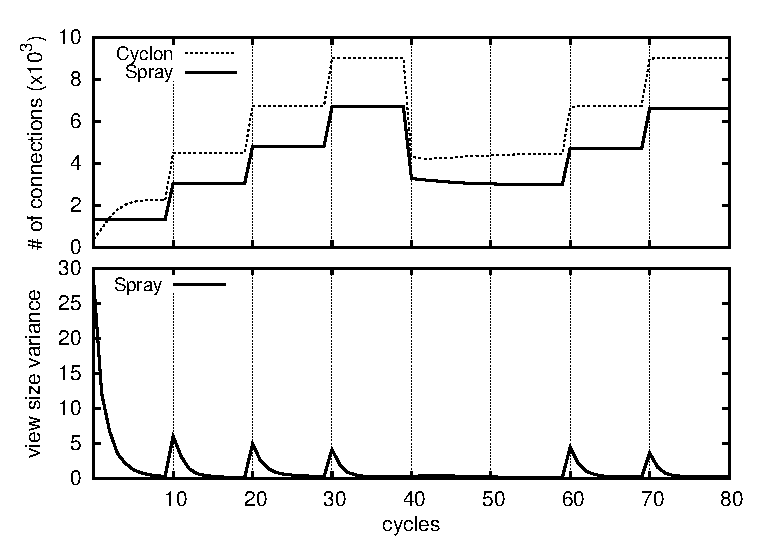
\includegraphics[width=0.47\textwidth]{img/spray/churn.eps}}
  \hspace{10pt}
  \subfloat[Figure B][\label{fig:spray:churnB}The x-axis denotes the
  elapsed time in cycles. The y-axis denotes the average partial view size.]{
    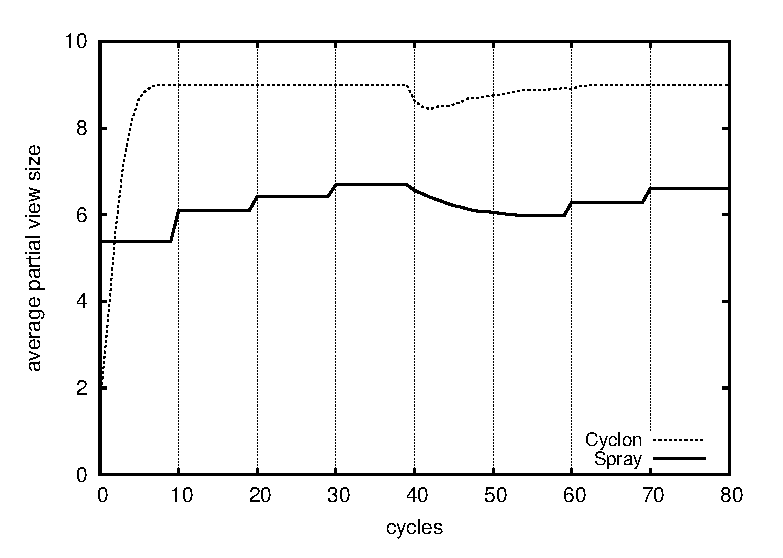
\includegraphics[width=0.47\textwidth]{img/spray/avgpv.eps}}
  \caption{\label{fig:spray:churn}\CYCLON (partial view size configured to 9)
    and \SPRAY in a dynamic network. 2.5k peers join the network at cycles $0$,
    $10$, $20$, and $30$. Then 5k peers leave at cycle $40$. Finally 2.5k peers
    join at cycles $60$ and $70$. The final network contains 10k members.}
\end{figure*}

\ \\

\begin{asparadesc}
\item [Objectif:] Montrer comment l'influence de l'adaptabilité sur un réseau
  dont la taille varie au court du temps.
\item [Description:] Cette expérimentation se concentre sur un réseau dynamique
  dont les membres rejoignent et quittent le système lorsqu'ils le
  souhaitent. Les exécutions concernent les protocoles d'échantillonnage \CYCLON
  et \SPRAY. La configuration de \CYCLON cible un réseau de taille 8.1k
  pairs. Ainsi, les vues partielles sont trop grandes lors de cette simulation
  qui implique au maximum 1k pairs. Lors de la première moitié de la simulation,
  4 groupes successifs comportant 250 pairs rejoignent le réseau. L'intervalle
  de temps entre ces entrées groupées est de 10 cycles. Ainsi, le réseau
  initialement vide contient 1k pairs au bout de 40 cycles. Ensuite, la moitié
  des membres du réseau le quitte (500 pairs). Enfin, 2 groupes de 250 pairs
  rejoignent le réseau à nouveau faisant passer la taille de celui-ci à 1k
  pairs. Les mesures concernent
  \begin{inparaenum}[(i)]
  \item le nombre de connexions dans le réseau au cours des cycles,
  \item la variance de la taille des vues partielles au cours des cycles,
  \item la taille moyenne des vues partielles au cours du temps.
  \end{inparaenum}
\item [Résultat:] La figure~\ref{fig:spray:churn} montre les résultats de cette
  expérimentation. L'axe des abscisses représente les cycles (i.e. une mesure
  arbitraire de temps). La partie haute de la figure~\ref{fig:spray:churnA}
  montre le nombre de connections établies dans le réseau (échelle
  $\times 10^3$) tandis que la partie basse de la figure montre la variance de
  taille des vues partielles parmis les pairs. En ce qui concerne \SPRAY, nous
  observons qu'à chaque groupe rejoignant le réseau, le nombre de connections
  augmente afin de refléter cette augmentation. Ces observations concordent avec
  les mesures sur la variance. En effet, à chaque groupe rejoignant le réseau,
  la variance augmente soudainement. Ensuite, elle décroît exponentiellement et
  converge vers 0 en moins de 10 cycles. La variance est plus élevée lorsque la
  taille du réseau est basse. Par exemple, le premier groupe de 250 pairs
  conduit à la plus forte hausse de variance. Au $40^{ème}$ cycle, la moitié des
  pairs quittent le réseau. Approximativement la moitié des connections sont
  supprimées mais n'influent pas sur la variance. Les 10 cycles suivant montre
  une très faible diminution du nombre d'arcs. Enfin, de nouveaux groupes de
  pairs sont réintroduits dans le réseau et mène au même conclusions que
  précédemment. \CYCLON montre le même genre de comportement. Néanmoins, le
  nombre d'arcs est invariablement supérieurs à celui de \SPRAY (entre 1000 et
  2500 connexions supplémentaires). La figure~\ref{fig:spray:churnB} montre la
  taille moyenne des vues partielles de \SPRAY et de \CYCLON. Comme prévu,
  \CYCLON converge immédiatement vers la taille de vue partielle planifiée lors
  de sa configuration (9 voisins). À l'opposé, la taille de vue partielle
  moyenne de \SPRAY augmente logarithmiquement tandis que la taille du réseau
  augmente. Lorsque les départs de pairs surviennent au cycle 40, \CYCLON
  supprime les liens morts tout en remplissant les vues partielles afin
  d'atteindre la taille de vue partielle de sa configuration initiale. \SPRAY
  supprime seulement les arcs nécessaire afin de refléter la nouvelle taille
  réseau. À la fin de la simulation, les pairs utilisant \SPRAY ont une vue
  partielle contenant 6.6 voisins en moyenne (rappel: $\ln(1000)\approx 6.9$).
\item [Explication:] Puisque les vues partielles de \SPRAY s'adaptent à la
  taille du réseau, le nombre de connexions augmente lorsque des membres
  s'ajoute au réseau. Les pics de variance correspondent à la partie du
  protocole où les pairs rejoignent le réseau. Cette disparité provient du fait
  que les nouveaux arrivant commencent avec une petite vue partielle. Les pics
  sont plus petits lorsque le réseau est plus grand. En effet, les pairs étant
  présent avant que le nouveau groupe rejoigne le réseau ont eu quelques cycles
  d'échanges afin d'équilibrer leur vue partielle. Par conséquent, le poids des
  nouveaux arrivant est proportionnellement plus faible. Le départ des 500 pairs
  au cycle 40 ne perturbe pas la variance car ils sont effectués de manière
  aléatoire. Ainsi, aucun pair ne souffre plus qu'un autre des départs. La très
  petite décroissance du nombre d'arcs après les départs est due au fait que les
  pairs restant réalisent que les pairs sont injoignables seulement après
  quelques cycles. 
\end{asparadesc}


\begin{figure}
  \centering
  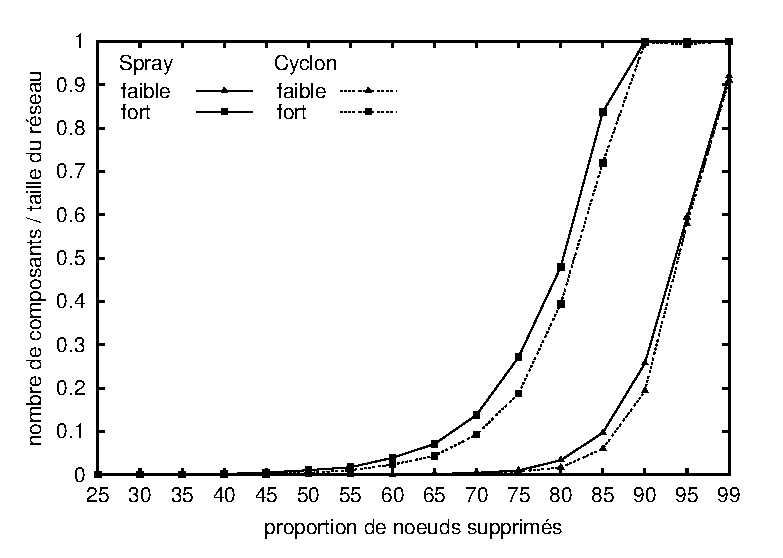
\includegraphics[width=.8\textwidth]{img/spray/resilience.eps}
  \caption{\label{fig:spray:resilience}Robustness of \CYCLON and \SPRAY to
    massive failures. The x-axis denotes the percentage of peers removed at once
    in a network containing 10k members. The y-axis denotes the number of
    components over the current network size (after the removals). The
    measurements concern the weak and strong components which basically means
    the number clusters in undirected or directed graph respectively.}
\end{figure}

\begin{asparadesc}
\item [Objectif:] Montrer que \SPRAY and \CYCLON sont tous deux robustes aux
  défaillances massives.
\item [Description:] Compter le nombre de composantes fortement connexes dans un
  réseau permet d'estimer la surface atteignable par les protocoles de
  dissémination d'informations. Par exemple, il y a deux composantes fortement
  connexes dans un réseau dont une partie peut atteindre l'autre sans que
  l'inverse soit vrai. Compter le nombre de composantes faiblement connexes dans
  une réseau permet d'estimer le moment où celui-ci n'est plus réparable. Un
  réseau est réparables si après quelques échanges de vues partielles, les
  informations peuvent être disséminées à tous les participants encore dans le
  réseau. \CYCLON est configuré pour obtenir des vues partielles contenant 9
  voisins. Le réseau compte 10k membres. Nous effectuons les suppressions de
  pairs après convergence des approches. Nous supprimons les pairs en une fois,
  allant de 25\% à 95\% par paliers de 5\% ce qui représente 16 exécutions par
  approche. La dernière mesure est effectuée à 99\% de suppressions. Les mesures
  sont effectuées immédiatement après les suppressions. Ces dernières concernent
  un pourcentage de pairs aléatoirement choisis parmi les 10k pairs.
\item [Résultat:] La figure~\ref{fig:spray:resilience} montre le ratio de
  composantes fortement/faiblement connexes du réseau après les suppressions de
  pairs. Tout d'abord, la figure montre que les deux protocoles
  d'échantillonnage de pairs, \SPRAY et \CYCLON, ne souffrent de comportement
  défaillant qu'après un haut pourcentage de suppressions, \CYCLON étant
  légèrement meilleur dans ce cas. La figure~\ref{fig:spray:resilience} montre
  que la dissémination d'informations (les composantes fortement connexes)
  commencent se dégrader lentement dès 45\%, et plus rapidement à
  70\%. Heureusement, la figure~\ref{fig:spray:resilience} nous montre aussi que
  ces approches sont capables de se réparer de ce clustering jusqu'à de haut
  taux de suppressions. En effet, les composantes faiblement connexes ne
  commencent à augmenter qu'à partir de 70\%, ce qui signifie que des parties du
  réseau sont complètement disjointes et donc, hors de toute possibilité de
  réparation.
\item [Explication:] Les protocoles d'échantillonnage de pairs \CYCLON et \SPRAY
  affichent de très similaires résultats car \CYCLON est configuré pour une
  taille de réseau de 10k pairs, tandis que \SPRAY s'ajuste automatiquement à
  cette taille de réseau. Par conséquent, leur nombre d'arcs est très
  proche. Ici, \CYCLON possède légèrement plus de connexions (car \SPRAY possède
  une part d'aléatoire) et aucun doublon dans les vues partielles (\SPRAY
  possède un faible taux de doublons,
  cf. Figure~\ref{fig:spray:duplicates}). Afin de mettre en dangers la
  dissémination d'information, il est nécessaire de supprimer un fort taux de
  pairs. En effet, chaque pair revêt grossièrement la même importance que son
  voisin. Ainsi, supprimer des pairs aléatoirement parmi ceux-ci n'affectent pas
  énormément le réseau en entier. Le réseau est capable de se réparer car les
  protocoles d'échantillonnage ne dépendent que d'arcs unidirectionnels pour
  fonctionner. Ainsi, s'il subsiste un lien entre deux composantes fortement
  connexes, les échanges de vues partielles permettent de réparer cela.
\end{asparadesc}


\begin{figure}
  \centering
  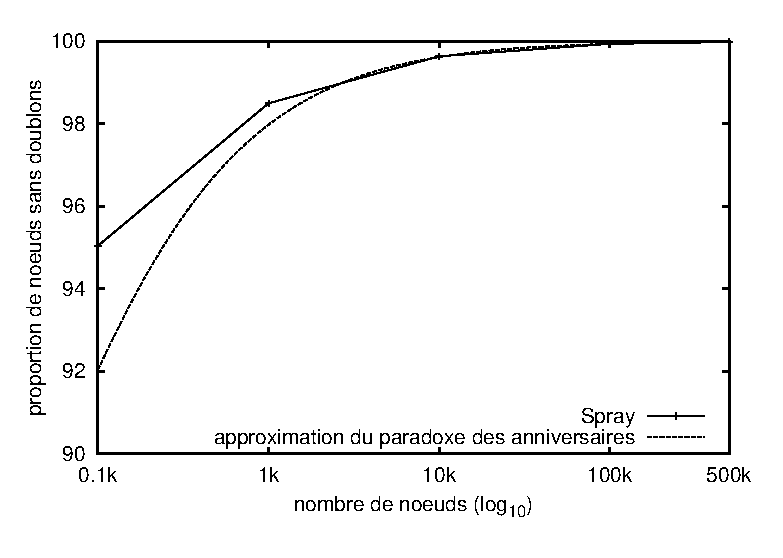
\includegraphics[width=.8\textwidth]{img/spray/duplicates.eps}
  \caption{\label{fig:duplicates}Duplicates in networks of different size: the
    $\log_{10}$-scaled x-axis denotes the network size while y-axis denotes the
    proportion of peers without any duplicates in their partial view.}
\end{figure}

\begin{figure}
  \centering 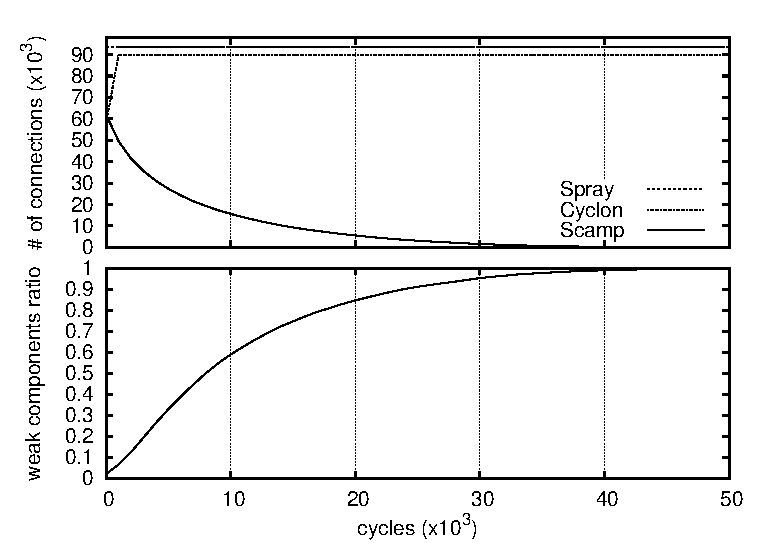
\includegraphics[width=.8\textwidth]{img/spray/degen.eps}
  \caption{\label{fig:degeneration}\CYCLON, \SCAMP, and \SPRAY in network
    subject to failures in the connection establishments. The x-axis denotes
    the elapsed time in cycles ($10^3$-scaled). The y-axis of the top figure
    denotes the global number of arcs ($10^3$-scaled). The y-axis of the bottom
    figure denotes the ratio of weak components over the current network size.}
\end{figure}

%%% Local Variables:
%%% mode: latex
%%% TeX-master: "../../paper"
%%% End:
